\documentclass[tikz,border=8pt]{standalone}
% Shared look for every TikZ diagram. Load with \input{../../tools/tikz-style.tex}
\usepackage[T1]{fontenc}
\usepackage{lmodern}
\renewcommand{\sfdefault}{lmr}  % diagrams use the same serif as the text
\usetikzlibrary{arrows.meta, positioning, shapes.geometric, calc, fit, backgrounds}
\definecolor{cblue}{HTML}{4C78A8}
\definecolor{corange}{HTML}{F58518}
\definecolor{cgreen}{HTML}{54A24B}
\definecolor{cred}{HTML}{E45756}
\definecolor{cpurple}{HTML}{B279A2}
\definecolor{cgrey}{HTML}{6B6B6B}
\tikzset{
  every picture/.style={font=\sffamily, line width=1.2pt},
  box/.style={draw=#1, fill=#1!12, rounded corners=4pt, align=center, inner sep=7pt, minimum height=1.1cm},
  box/.default=cgrey,
  arrow/.style={-{Stealth[length=3mm]}, draw=cgrey, line width=1.4pt},
  title/.style={font=\sffamily\bfseries\Large},
  note/.style={font=\sffamily\small, text=cgrey, align=center},
}
\AtBeginDocument{\hyphenpenalty=10000 \exhyphenpenalty=10000}

\begin{document}
\begin{tikzpicture}[b/.style={box=cblue, minimum width=4.6cm}, g/.style={box=cgrey, minimum width=4.6cm},
  r/.style={box=cred, minimum width=4.6cm}, gr/.style={box=cgreen, minimum width=4.6cm}, o/.style={box=corange, minimum width=4.6cm}]
  \node[r] (f0) at (0,0) {stage 1: $F_0 = \log\dfrac{\#\,1\text{s}}{\#\,0\text{s}}$\\(log-odds)};
  \node[o] (p) at (0,-2.2) {probability: $p = \sigma(F) = \dfrac{1}{1+e^{-F}}$};
  \node[g] (res) at (0,-4.3) {pseudo-residuals: $r = y - p$};
  \node[gr] (tree) at (7,-4.3) {regression tree on $r$};
  \node[gr] (leaf) at (7,-2.2) {leaf value in log-odds:\\$\gamma = \dfrac{\sum r}{\sum p(1-p)}$};
  \node[r] (upd) at (7,0) {update the log-odds:\\$F \leftarrow F + \eta \cdot \gamma$};
  \draw[arrow] (f0) -- (p); \draw[arrow] (p) -- (res); \draw[arrow] (res) -- (tree); \draw[arrow] (tree) -- (leaf);
  \draw[arrow] (leaf) -- (upd);
  \draw[arrow, dashed] (upd.west) -- node[note, above, sloped] {next stage} (p.north east);
\end{tikzpicture}
\end{document}
